% DO NOT COMPILE THIS FILE DIRECTLY!
% This is included by the other .tex files.

\section*{Outline}
\frame{\tableofcontents}


\section{Introduction}
\begin{frame}[t,fragile]{\textbf{Introduction}}
Test
\end{frame}

\section{Controller overview}
\begin{frame}[t,fragile]{Rules}
\begin{enumerate}
  \item If the \textbf{nest} has been \textbf{left}, and \textbf{no} chain beacon have been already \textbf{sensed}, after $t_{ns}$ time step, decide with probability $p_{btoe}$ to stop and become a \emph{chain end (E)}.
  \item If the \textbf{nest} has been \textbf{left}, and \textbf{exactly one} chain beacon has been \textbf{sensed} at a distance greater than $d_{chain}$, stop and become a \emph{chain end (E)}.
  \item If a \textbf{chain end (E)} has \textbf{more than one} neighboring\textbf{ beacon}, but \textbf{less than three}, then it changes its state to \emph{chain member (M)}.
  \item If a \textbf{chain member (M)} has \textbf{more than two} neighboring \textbf{beacons}, then it changes its state to \emph{chain junction (J)}.
  \item The chain identifier of a new beacon is determined by incrementing of one unit the chain id of the closest beacon.
\end{enumerate}

\end{frame}

\begin{frame}[t,fragile]{\textbf{Chain example}}
\begin{center}
\begin{tikzpicture}[shorten >=1pt,node distance=2cm,on grid,auto] 
   \node[state,accepting] (R1)   {$E_0$}; 
   \node[state,thick] (R2) [right=of R1] {$M_1$};
   \node[state,thick] (R3) [right=of R2] {$J_2$};
   \node[state,accepting,thick] (R4) [above right=of R3] {$E_3$};
   \node[state,thick] (R5) [below right=of R3] {$M_3$};
   \node[state,accepting,thick] (R6) [right=of R5] {$E_4$};
    \path[]
    (R1) edge (R2)
    (R2) edge (R3)
    (R3) edge (R4)
    (R3) edge (R5)
    (R5) edge (R6);
\end{tikzpicture}
\captionof{figure}{Chain example with nodes labeling and id}
\end{center}
\end{frame}

\section{Controller details}
\begin{frame}[t,fragile]{\textbf{State machine}}
\begin{tiny}
%\begin{center}
\begin{tikzpicture}[scale=0.2,shorten >=1pt,node distance=3cm,on grid,auto] 
   \node[state,initial] (EN)   {Exit Nest}; 
   \node[state,thick] (EX) [below=of EN] {Explorer};
   \node[state,thick] (EC) [right=of EN] {Chain Following};
   \node[state,accepting,thick] (SR) [right=of EC] {Spot Reached};
   \node[state,accepting,thick] (CE) [below =of EC] {Chain End};
   \node[state,accepting,thick] (CM) [right=of CE] {Chain Member};
   \node[state,accepting,thick] (CJ) [below right=of CM] {Chain Junction};
   \node [draw,rectangle,text width=4cm] (box) at (0,-26) {%
    $n_b$ : Number of beacons
     
    $d_{cb}$ : Distance to closest beacon
     
    $P_{etob}$ : Probability to become beacon
     
    $d_c$ : Chain distance
    };
    \path[->] 
    (EN) edge [bend right]  node [left,text width=2cm]  {Out of nest $\wedge \text{ } n_b = 0$} (EX)
         edge [bend left]  node [above]  {$n_b >0$} (EC)
    (EX) edge [bend left]  node [above,rotate=45]  {$n_b >0$} (EC)
         edge [bend right]  node [below,text width=1.3cm]  {$n_b = 0 \text{ } \wedge$ Out of Nest $\wedge \text{ } P_{etob}$} (CE)
          edge  node [above left,rotate=90]  {In Nest} (EN)
    (CE) edge node  {$n_b > 1$} (CM)
           edge [bend left] node [below left,text width=0.7cm]  {$d_{cb} < 30[cm]$} (EC)
    (CM) edge [bend left] node [text width=2cm] {$n_b > 2$} (CJ)
    (EC) edge  node [above]  {In Nest} (EN)
           edge  node [above,rotate=45]  {$n_b > 1 \text{ } \wedge$ Out of Nest} (EX) 
           edge [bend left] node [right,text width=1.3cm] {$n_b = 1 \text{ } \wedge$ Out of Nest $\wedge \text{ } d_{cb} > d_c$} (CE)
           edge  node {On spot} (SR);
\end{tikzpicture}
%\captionof{figure}{Implemented FSM for the \emph{s-bot} chain formation behavior}
%\end{center}
\end{tiny}
\end{frame}

\section{Results}
\begin{frame}[t,fragile]{\textbf{Robots in chain}}
\begin{minipage}{.47\textwidth}
\centering
\includegraphics[width=\textwidth,keepaspectratio]{{../Results/50Trials/Panel1}.pdf}
\end{minipage}%
\hspace{0.15cm}
\begin{minipage}{.47\textwidth}
\centering
\includegraphics[width=\textwidth,keepaspectratio]{{../Results/50Trials/Panel2}.pdf}
\end{minipage}
\end{frame}


\begin{frame}[t,fragile]{\textbf{Completion time}}
\begin{minipage}{.47\textwidth}
\centering
\includegraphics[width=\textwidth,keepaspectratio]{{../Results/50Trials/Panel3}.pdf}
\end{minipage}%
\hspace{0.15cm}
\begin{minipage}{.47\textwidth}
\centering
\includegraphics[width=\textwidth,keepaspectratio]{{../Results/50Trials/Panel4}.pdf}
\end{minipage}
\end{frame}

\begin{frame}[t,fragile]{\textbf{Correlation}}
\begin{center}
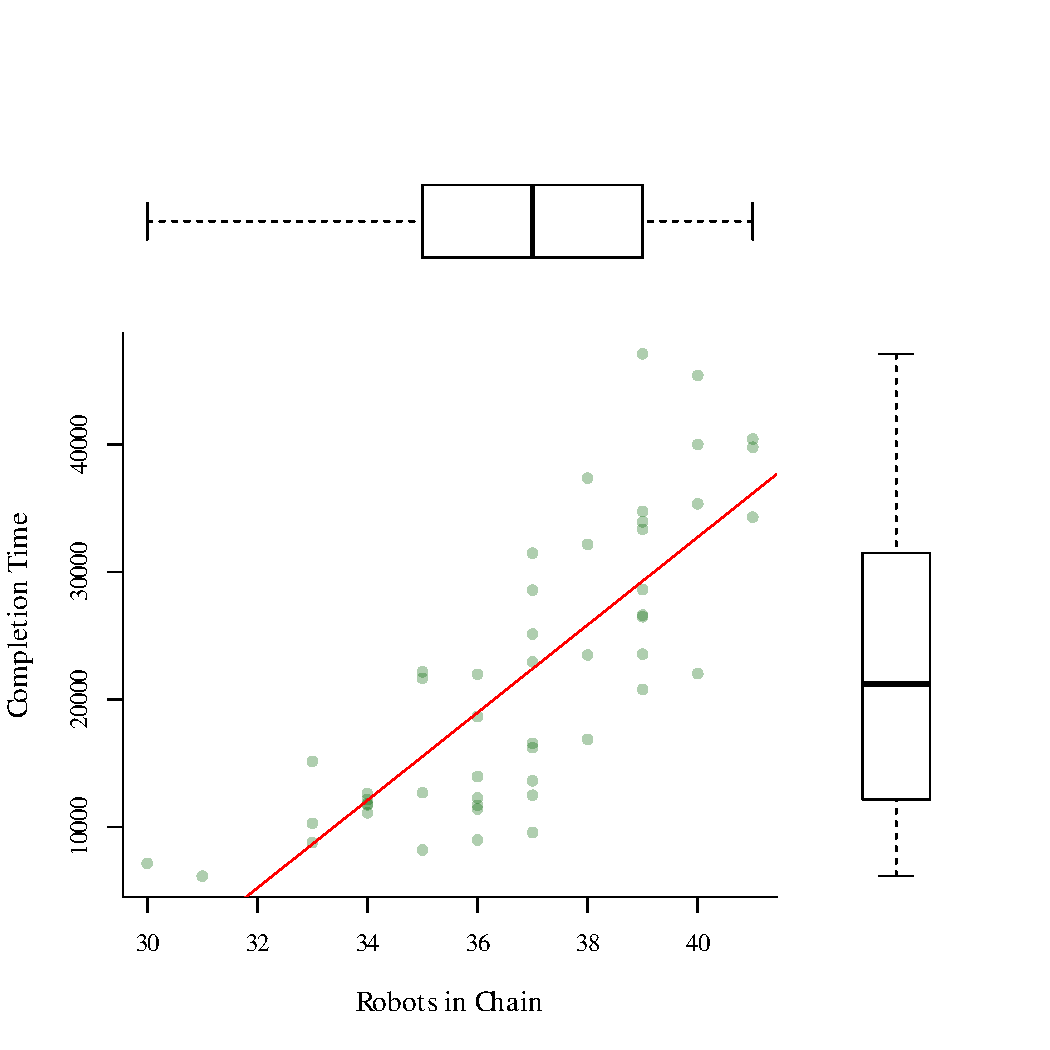
\includegraphics[width=0.7\textwidth,keepaspectratio]{{../Results/50Trials/ResultsDistribution}.pdf}  
\end{center}
\end{frame}

% \section{Context of the research}
% \begin{frame}[t,fragile]{Research context}
% The evaluation of interactive segmentation is generally done by means of user experimentation.\newline
% This method is effective, but also labor-intensive and time-consuming.\newline 
% The paper proposes an automated approach imitating human behaviour, evaluating it using 4 different algorithms:
% \begin{enumerate}
% \item \textbf{BPT: }Interactive segmentation using Binary Partition Trees
% \item \textbf{IGC: } Interactive Graph Cuts
% \item \textbf{SRG: } Seeded Region Growing 
% \item \textbf{SIOX: } Simple Interactive Object Extraction
% \end{enumerate}
% These algorithms provide a good coverage of the underlying algorithmic approaches described in the literature for
% object extraction from natural scenes.

% \end{frame}

% \section{Theoretical notions}

% \begin{frame}[t,fragile]{User-based segmentation}
% \begin{center}
% \includegraphics[height=.8\textheight,keepaspectratio]{AutomationSchema}
% \end{center}
% \end{frame}

% \begin{frame}[t,fragile]{Strategies overview}
% \begin{itemize}
% \item \textbf{Strategy 1 -} Deterministic choice of ground truth objects centers as seed points.
% \item \textbf{Strategy 2 -} Non-deterministic choice of seeds points with distance-proportional probability.
% \item \textbf{Strategy 3 -} Computation of the shortest seed line defining an acceptable segmentation.
% \item \textbf{Strategy 4 -} Computation of the shortest seed line defining an acceptable segmentation with preference for those passing near the center of the object.
% \end{itemize}
% \end{frame}

% \begin{frame}[t,fragile]{Automated Strategy 1 - Overview}
% Seed points are chosen in a way that :
% \begin{itemize}
%   \item \textbf{(Initialization) -}Intuitively, points closer to the center of the ground truth object are marked as object point, while points clearly outside of it are marked as background
%   \item \textbf{(Update) -} Update seed points are chosen within large misclassified areas
% \end{itemize}
% \textbf{Strong points :}
% \begin{itemize}
%   \item Efficient computation using fast 2D Euclidian distance. 
%   \item Determinism.
%   \item Useful baseline for comparisons.
% \end{itemize}
% \textbf{Weak points :}
% \begin{itemize}
%   \item Determinism does not allow to test the robustness of the strategy.
%   \item Seeds have the form of pixel blobs instead of curves.
% \end{itemize}
% \end{frame}


% \begin{frame}[t,fragile]{Automated Strategy 2 - Overview}
% The strategy is similar to the previous one, the main difference being a non deterministic choice of the points according to a probability distribution which is proportional
% to the distance of points within the candidate set to points outside this set. \newline
% \textbf{Strong points :}
% \begin{itemize}
%   \item Efficient computation using inversion method to compute the probability.
%   \item Non-Determinism allows to test repeatability, hence robustness.
% \end{itemize}
% \textbf{Weak points :}
% \begin{itemize}
%   \item Seeds have the form of pixel blobs instead of curves.
% \end{itemize}
% \end{frame}

% \begin{frame}[t,fragile]{Automated Strategy 1-2 - Example}
% \begin{center}
% \includegraphics[height=.8\textheight,keepaspectratio]{Strategy1Ex}
% \end{center}
% \end{frame}


% \begin{frame}[t,fragile]{Automated Strategy 3 - Overview}
% The seed set will have the form of an automatically generated line, obtained by applying Dijkstra's shortest path algorithm on the adjacency graph of the candidate pixels.
% The line will be eventually expanded using a brush function to ensure a better coverage of the object.\newline
% \textbf{Strong points :}
% \begin{itemize}
%   \item Efficient computation of connection relationship and shortest path using Dijkstra's algorithm.
%   \item Seed line define a better coverage of the ground truth object than pixel blobs.
% \end{itemize}
% \textbf{Weak points :}
% \begin{itemize}
%   \item Shortest seed line tends to be closer to the border than desired.
% \end{itemize}
% \end{frame}

% \begin{frame}[t,fragile]{Automated Strategy 3 - Example}
% \begin{center}
% \includegraphics[height=.5\textheight,keepaspectratio]{Strategy3Ex}
% \end{center}
% \end{frame}

% \begin{frame}[t,fragile]{Automated Strategy 4 - Overview}
% This strategy is identical to the previous one, except for the weight assigned to each edge in the adjacency graph, which is modified in order to produce
% seed lines which pass closer to the center of the ground truth object.\newline
% \textbf{Strong points :}
% \begin{itemize}
%   \item Efficient computation of connection relationship and shortest path using Dijkstra's algorithm.
%   \item Seed line define a better coverage of the ground truth object than pixel blobs.
% \end{itemize}
% \textbf{Weak points :}
% \begin{itemize}
%   \item Shortest seed line tends to be closer to the border than desired.
% \end{itemize}
% \end{frame}

% \begin{frame}[t,fragile]{Automated Strategy 3 - Example 1}
% \begin{center}
% \includegraphics[height=.5\textheight,keepaspectratio]{Strategy3Ex2}
% \end{center}
% \end{frame}

% \begin{frame}[t,fragile]{Automated Strategy 3 - Example 2}
% \begin{center}
% \includegraphics[height=.7\textheight,keepaspectratio]{Strategy4Ex}
% \end{center}
% \end{frame}

% \section{Results Analysis}
% \begin{frame}[t,fragile]{Evaluation method}
% Given an input image and the corresponding ground truth:
% \begin{enumerate}
% \item Select strategy and algorithm.
% \item Process image according to strategy and algorithm.
% \item Compute object accuracy and border accuracy.
% \item Update seeds.
% \item If maximum step number has been reached stop, else goto 2.
% \end{enumerate}
% \begin{itemize}
%   \item Non deterministic strategy are rerunned 5 times in order to evaluate repeatability.
%   \item The maximum number of steps is equal to 100, which is unrealistic compared to human interaction, to allow stabilization of the results and to observe the strategy behavior over a long run.
%   \item Object and border accuracy will result in a time series of values.
%   \item Accuracy =  $\frac{TruePositive}{TruePositive+FalsePositive+FalseNegative}$ (Jaccard Index)
% \end{itemize}
% \end{frame}

% \begin{frame}[t,fragile]{Evaluation metrics}
% \begin{itemize}
%   \item \textbf{(Profile) - Time-Accuracy Profile } Average accuracy profile across time.
%   \item \textbf{(Aggregate) - Final Accuracy } Accuracy achievable across a reasonable amount of time.
%   \item \textbf{(Aggregate) - Integrated Accuracy } Accuracy integrated over time series data expanded in order to be comparable 
% \end{itemize}
% \begin{itemize}
%   \item These metrics can be averaged across all the object in the dataset to assess overall system performance.
%   \item Integrated accuracy is computed as a discrete summation of the area below the expanded time series.
%   \item Useful because it can be easily normalized with respect to the unity rectangle and briefly express the trend of average accuracy.
%   \item  Must be computed also for user interaction where steps are not unit spaced (i.e resampling or trapezoid rule).
% \end{itemize}
% \end{frame}

% \begin{frame}[t,fragile]{User Interaction Results}
% \begin{center}
% \includegraphics[height=.8\textheight,keepaspectratio]{MeanAccuracyUser}
% \end{center}
% \end{frame}

% \begin{frame}[t,fragile]{Automation Results - Accuracy Profile}
% \begin{center}
% \includegraphics[height=.8\textheight,keepaspectratio]{MeanAccuracyAutomation}
% \end{center}
% \end{frame}

% \begin{frame}[t,fragile]{Automation Results - Final Accuracy}
% \begin{center}
% \includegraphics[height=.7\textheight,keepaspectratio]{MeanAccuracyFinal}
% \end{center}
% \end{frame}

% \begin{frame}[t,fragile]{Automation Results - Integrated Accuracy}
% \begin{center}
% \includegraphics[height=.7\textheight,keepaspectratio]{MeanAccuracyIntegrated}
% \end{center}
% \end{frame}

% \begin{frame}[t,fragile]{Correlation metrics}
% \begin{itemize}
%   \item \textbf{Pearson's product-moment coefficient} 
%   \item \textbf{Spearman's $\rho$ rank coefficient}
% \end{itemize}
% \begin{itemize}
%   \item User (time-based) and automated (step-based) data must be aligned to perform correlation analysis.
%   \item Step-accuracy correlation analysis is limited to 60 step, because of results stabilization and limited number of user interactions.
%   \item Aggregated measures are averaged across different users (for human interaction) or different runs (for non-deterministic strategies) before performing correlation analysis.
%   \item High correlation between user and automated accuracy profile will show that the proposed method is well-emulating human behavior. 
% \end{itemize}
% \end{frame}

% \begin{frame}[t,fragile]{Automation Results - Step-accuracy correlation}
% \begin{center}
% \includegraphics[height=.6\textheight,keepaspectratio]{StepwiseCorrelation}
% \end{center}
% \end{frame}

% \begin{frame}[t,fragile]{Automation Results - Aggregate values correlation}
% \begin{center}
% \includegraphics[height=.7\textheight,keepaspectratio]{AggregateCorrelation}
% \end{center}
% \end{frame}

% \begin{frame}[t,fragile]{Conclusions}
% \begin{itemize}
% \item All the strategies have lead to results which are similar to those obtained with user segmentation.
% \item Strategy 3 and 4 have shown to be the most effective strategies at approximating real user input (highest rank correlation), with strategy 4 time accuracy profile having the closer visual correspondence with respect to user experiments one. 
% \item User evaluation is still the most effective way to evaluate interactive segmentation.
% \item Automated evaluation could provide useful and informative results whenever user test cannot be performed (e.g. due to high time consumption).
% \end{itemize}
% \end{frame}
